\documentclass[12pt]{article}

\usepackage{amsmath}
\usepackage{amsfonts}
\usepackage{float}
\usepackage{fancyhdr}
\usepackage{graphicx}
\usepackage[colorlinks=true,linkcolor=blue, citecolor=red]{hyperref}
\usepackage{url}
\usepackage[top=1.3in, left=1.2in, right=.95in, bottom=1.3in]{geometry}
\usepackage[spanish]{babel}
\usepackage{lipsum}
\usepackage{blindtext}



% For algorithm
\usepackage{algorithm}
\usepackage{algpseudocode}

% ============ CODE ============
\usepackage{listings}
\usepackage{xcolor}
\definecolor{codegreen}{rgb}{0,0.6,0}
\definecolor{codegray}{rgb}{0.5,0.5,0.5}
\definecolor{codepurple}{rgb}{0.58,0,0.82}
\definecolor{backcolour}{rgb}{0.95,0.95,0.92}

% Styling for the code.
\lstdefinestyle{mystyle}{
    backgroundcolor=\color{backcolour},   
    commentstyle=\color{codegreen},
    keywordstyle=\color{magenta},
    numberstyle=\tiny\color{codegray},
    stringstyle=\color{codepurple},
    basicstyle=\ttfamily\footnotesize,
    breakatwhitespace=false,         
    breaklines=true,                 
    captionpos=b,                    
    keepspaces=true,                 
    numbers=left,                    
    numbersep=5pt,                  
    showspaces=false,                
    showstringspaces=false,
    showtabs=false,                  
    tabsize=2
}
\lstset{style=mystyle}

% Disable indentation on new paragraphs
\setlength{\parindent}{0pt}

% Optional: graphic path
% \graphicspath{PATH_TO_GRAPHIC_FOLDER}

% To use Times font family, uncomment this row
% \usepackage{mathptmx}

% To use roman section / subsection, uncomment these rows
% \renewcommand{\thesection}{\Roman{section}}
% \renewcommand{\thesubsection}{\thesection.\Roman{subsection}}

% Define course name, report name and report title.


\newcommand{\coursename}{Escuela Profesional de Ingeniería de Sistemas e Informática} 


%%%%%%INICIO CARATULA%%%%%%%%%%%%%%%%%%%

%informe laboratorio numero
\newcommand{\reportname}{Informe laboratorio N° 1} 

%titulo del informe
\newcommand{\reporttitle}{Implementación y comparación de tiempo de desempeño de los principales siete algoritmos de ordenamiento } 

\newcommand{\studentname}{
Jesús Ronald Rosales Roca \\
 
}
\newcommand{\teachername}{Honorio Apaza Alanoca}

%\newcommand{\leftfooter}{\LaTeX\ by \href{https://github.com/trhgquan}{Quan, Tran Hoang}}


%%%%%% FIN CARATULA%%%%%%%%%%%%%%%%%%%



% ============ HEADER AND FOOTER ============
% Header length
\setlength{\headheight}{29.43912pt}

% Footer page number would be on the lower-right corner
\pagestyle{fancy}
\fancyfoot{}
\fancyfoot[R]{Pag. \thepage}

\lhead{}
\rhead{
Universidad Nacional de Moquegua\\
\coursename
}
%\lfoot{\leftfooter}

% ============ DOCUMENT ============
\begin{document}
\begin{titlepage}
\newcommand{\HRule}{\rule{\linewidth}{0.5mm}}
\centering

\textsc{\Large \textbf{UNIVERSIDAD NACIONAL DE MOQUEGUA}}\\[0.5cm]
\textsc{\Large Facultad de Ingeniería y Arquitectura }\\[0.5cm]
\textsc{\large Escuela Profesional de Ingeniería de Sistemas e Informática}\\[1.5cm]


\includegraphics[scale=.25]{img/image.png}\\[0.2cm] 

%\textsc{Titulo del trabajo:}\\[0.5cm]

\noindent\hrulefill \\[0.5cm]
{ 
\Large{\bfseries{\reporttitle}}\\[0.5cm]
\large{\bfseries{\reportname}}
}\\[0.4cm]
\noindent\hrulefill \\[0.5cm]

%\textbf{\large Nombres y Apellidos: \coursename}\\[0.5cm]


\begin{minipage}[t]{0.4\textwidth}
\begin{flushleft} \large
\emph{Estudiante:}\\
\studentname
\end{flushleft}
\end{minipage}
~
\begin{minipage}[t]{0.4\textwidth}
\begin{flushright} \large
\emph{Profesor:} \\
\teachername
\end{flushright}
\end{minipage}\\[2cm]

{\large \today}\\[2cm]



\vfill
\end{titlepage}
	
	
\tableofcontents
\pagebreak


\section*{Introducción}
\addcontentsline{toc}{section}{Introducción}


La organización eficiente de datos es un aspecto fundamental en el campo de la informática y la programación, ya que influye directamente en el rendimiento de las aplicaciones y sistemas. Los algoritmos de ordenamiento son herramientas esenciales que permiten estructurar conjuntos de datos en un orden específico, facilitando así su búsqueda y manipulación. En este sentido, la elección del algoritmo adecuado puede marcar la diferencia en la eficiencia de un programa, especialmente cuando se trabaja con grandes volúmenes de información.

Esta monografía se centra en la implementación y comparación de los siete algoritmos de ordenamiento más utilizados: Bubble Sort, Selection Sort, Insertion Sort, Counting Sort, Heap Sort, Merge Sort y Quick Sort. A través de un análisis detallado de cada uno de estos métodos, se busca no solo entender su funcionamiento, sino también evaluar su desempeño en diferentes escenarios. La importancia de este estudio radica en que, al comprender las características y limitaciones de cada algoritmo, los desarrolladores pueden tomar decisiones más informadas que optimicen el rendimiento de sus aplicaciones.

El objetivo principal de esta investigación es proporcionar una visión clara y concisa sobre los algoritmos de ordenamiento, destacando sus ventajas y desventajas, así como su aplicabilidad en situaciones prácticas. Además, se pretende contribuir al aprendizaje de los estudiantes de ingeniería de sistemas, ofreciendo un recurso que les permita profundizar en el tema y aplicar este conocimiento en sus futuros proyectos. A lo largo de este documento, se presentarán los resultados de las implementaciones realizadas, así como un análisis comparativo de los tiempos de ejecución, lo que permitirá establecer conclusiones sobre la eficiencia de cada algoritmo en función de diferentes variables.










\newpage
\section{Marco teórico}


\vspace{0.5cm}

\subsection{Los 7 algoritmos de ordenamiento en pseudocodigo}
Los algoritmos de ordenamiento constituyen una parte fundamental de las ciencias de la computación, siendo procesos sistemáticos diseñados para organizar elementos en una secuencia específica, típicamente en orden ascendente o descendente. La importancia de estos algoritmos radica en su aplicación ubicua en el procesamiento de datos y su rol crucial en la optimización de búsquedas y otras operaciones computacionales.

\vspace{2.5cm}

\begin{algorithm}
\caption{Pseudocodigo Bubble Sort}
\label{alg:label}
\begin{algorithmic}
\Function {bubblesort}{\textit{array[]},\textit{ n}}
\State $n \gets length(array)$
\For {$i = 0  \hspace{0.2cm} to \hspace{0.1cm} (n - 1)$}
\For {$j = 0  \hspace{0.2cm} to \hspace{0.1cm} (n - 1 - i)$}
\If {$array[j] > array \hspace{0.1cm}[j + 1]$}
\State $temp \gets array \hspace{0.1cm}[j + 1]$
\State $array \hspace{0.1cm}[j]\gets array \hspace{0.1cm} [j + 1]$
\State $array \hspace{0.1cm}[j+1]\gets temp$
\EndIf
\EndFor
\EndFor
\EndFunction
\end{algorithmic}
\end{algorithm}
\begin{algorithm}
\caption{Pseudocodigo Selection Sort}
\label{alg:label}
\begin{algorithmic}
\Function {selectionsort}
{\textit{array[]},\textit{ n}}
\State $n \gets length(array)$

\For {$i = 0  \hspace{0.2cm} to \hspace{0.1cm} n$}
\State $menor \gets i$
\For {$j = i + 1  \hspace{0.2cm} to \hspace{0.1cm} n$}
\If {$array[j] < array \hspace{0.1cm}[menor]$}

\State $menor \gets j$
\EndIf

\EndFor

\EndFor
\State $temp \gets array[menor]$
\State $array[menor] \gets array[i]$
\State $array[i] \gets temp$
\EndFunction
\end{algorithmic}
\end{algorithm}

\begin{algorithm}
\caption{Pseudocodigo Insertion Sort}
\label{alg:label}
\begin{algorithmic}
\Function {insertionsort}
{\textit{array[]},\textit{ n}}
\State $n \gets length(array)$

\For {$i = 0  \hspace{0.2cm} to \hspace{0.1cm} (n - 1)$}

\For {$j = 0  \hspace{0.2cm} to \hspace{0.1cm} i$}
\If {$array[i] < array \hspace{0.1cm}[j]$}

\State $cambia \gets array[i]$
\State $array[i] \gets array[j]$
\State $array[j] \gets cambia$
\EndIf

\EndFor

\EndFor

\EndFunction
\end{algorithmic}
\end{algorithm}



\begin{algorithm}
\vspace{1cm}
\caption{Pseudocodigo Counting Sort}
\label{alg:label}
\begin{algorithmic}
\Function {countingsort}
{\textit{array[]},\textit{ n}}
\State $n \gets length(array)$
\State $count \gets array[n] de 0$
\State $output \gets array[n]$

\For {$i = 0  \hspace{0.2cm} to \hspace{0.1cm} n - 1$}
\State $j \gets key(input[i])$
\State $count[j] \gets count[j] + 1$
\EndFor
\vspace{0.2cm}

\For {$i = 1  \hspace{0.2cm} to \hspace{0.1cm} n$}
\State $count[i] \gets count[i] + count[i - 1]$
\EndFor
\vspace{0.2cm}
\For {$i = 0  \hspace{0.2cm} to \hspace{0.1cm} n - 1$ \textbf{down to 0} }
\State $j \gets key(input[i])$
\State $count[j] \gets count[j] - 1$
\State $output[count[j]] \gets input[i]$
\EndFor

\textbf{return} output
\EndFunction
\end{algorithmic}
\end{algorithm}

\begin{algorithm}
\caption{Pseudocodigo Heap Sort}
\label{alg:label}
\begin{algorithmic}
\Function {heapify}
{\textit{array[]},\textit{ n},\textit{ i}}
\State $n \gets length(array)$
\State $max \gets i$
\State $lchild \gets 2i + 1$
\State $rchild \gets 2i + 2$


\If {$(lchild <= n \hspace{0.1cm} ) \And (array[i] < array[lchild])$}

\vspace{0.2cm}
\State $max \gets lchild$

\Else 
\State $max \gets i$
\EndIf
\If {$(rchild <= n \hspace{0.1cm} ) \And (array[max] < array[rchild])$}
\State $max \gets rchild$
\EndIf
\If {$max != i$}
\State $\textbf{swap(array[i], array[max])}$
\State  $\textbf{Heapify(A, n, max)}$
\EndIf

\EndFunction
\vspace{0.5cm}
\Function {heapify}
{\textit{array[]}}

\State $n \gets length(array)$

\For {$i = n/2\hspace{0.1cm} downto\hspace{0.1cm} 1$}
\State  $\textbf{Heapify(A, n, i)}$
\EndFor
\For {$i = n\hspace{0.1cm} downto\hspace{0.1cm} 2$}
\State $exchange array[1] with array[i]$
\State $array.heapsize \gets  array.heapsize
 - 1$
\State  $\textbf{Heapify(A, i, 0)}$
\EndFor
\EndFunction
\end{algorithmic}
\end{algorithm}



\begin{algorithm}
\caption{Pseudocodigo Merge Sort}
\begin{algorithmic}
\Function{mergesort}{\textit{array[]},\textit{ left},\textit{ right}}
    \If{$left < right$}
        \State mid $\gets \left( \text{left} + \text{right} \right) / 2$
        \State $mergesort(A, left, mid)$
        \State $mergesort(A, mid + 1, right)$
        \State $merge(A, left, mid, right)$
    \EndIf
\EndFunction
\vspace{0.5cm}
\Function{merge}{\textit{array[]},\textit{ left},\textit{ mid}, \textit{ right}}
    \State $n1 \gets mid - left + 1$
    \State $n2 \gets right - mid$
    \State $Create arrays L[0..n1-1] and R[0..n2-1]$

    \For{$i = 0 \To n1 - 1$}
        \State L[i] $\gets$ A[left + i]
    \EndFor
    \For{$j = 0 \To n2 - 1$}
        \State $R[j] \gets A[mid + 1 + j]$
    \EndFor

    \State i $\gets$ 0, j $\gets$ 0, k $\gets$ left
    \While{$i < n1 \And j < n2$}
        \If{$L[i] \leq R[j]$}
            \State $A[k] \gets L[i]$
            \State $i \gets i + 1$
        \Else
            \State $A[k] \gets R[j]$
            \State $j \gets j + 1$
        \EndIf
        \State $k \gets k + 1$
    \EndWhile

    \While{$i < n1$}
        \State $A[k] \gets L[i]$
        \State $i \gets i + 1$
        \State $k \gets k + 1$
    \EndWhile

    \While{$j < n2$}
        \State $A[k] \gets R[j]$
        \State $j \gets j + 1$
        \State $k \gets k + 1$
    \EndWhile
\EndFunction

\end{algorithmic}
\end{algorithm}

\begin{algorithm}
\caption{Pseudocodigo Quick Sort}
\label{alg:label}
\begin{algorithmic}
\Function {quicksort}
{\textit{array[]},\textit{ ini},\textit{ fin}}

\If{inicio < fin}
        \State pivote $\gets$ arr[inicio]
        \State $i \gets inicio + 1$
        \State $j \gets fin$

        \While{i $\leq$ j}
            \While{i $\leq$ j \textbf{and} arr[i] $\leq$ pivote}
                \State $i \gets i + 1$
            \EndWhile
            \While{i $\leq$ j \textbf{and} arr[j] $>$ pivote}
                \State $j \gets j - 1$
            \EndWhile
            \If{i $<$ j}
                \State temp $\gets$ arr[i]
                \State arr[i] $\gets$ arr[j]
                \State arr[j] $\gets$ temp
            \EndIf
        \EndWhile
        
        \State temp $\gets$ arr[inicio]
        \State arr[inicio] $\gets$ arr[j]
        \State arr[j] $\gets$ temp

        \State \Call{quickSort}{arr, inicio, j - 1}
        \State \Call{quickSort}{arr, j + 1, fin}
    \EndIf

\EndFunction
\end{algorithmic}
\end{algorithm}


\newpage






\section{Metodología}

\subsection{Revisión de literatura}

\begin{itemize}
    \item  Bubble Sort:
    Es uno de los algoritmos de ordenamiento más básicos y fundamentales en ciencias de la computación. Su nombre deriva de la forma en que los elementos "flotan" hacia sus posiciones correctas durante el proceso de ordenamiento, similar a burbujas subiendo a la superficie del agua.El algoritmo se basa en el principio de comparación e intercambio de elementos adyacentes. Opera realizando múltiples pasadas a través de una lista, comparando pares de elementos consecutivos y realizando intercambios cuando es necesario.
    \item Selection Sort:
    Es un algoritmo de ordenamiento que se destaca por su simplicidad conceptual y su planteamiento intuitivo. Su nombre proviene de su operación principal: la selección repetida del elemento mínimo del array no ordenado.El algoritmo se divide en dos partes: Una sublista ordenada que se construye de izquierda a derecha y una sublista no ordenada que contiene los elementos restantes.
    \item Insertion Sort:
    Se trata de un algoritmo trabaja de manera similar a cómo las personas ordenan cartas de juego en sus manos: Se toma una carta nueva, las comparamos con las cartas que ya tenemos ordenadas y la insertamos en su posición correcta de la lista.
    \item Counting Sort:
    Es un algoritmo de ordenamiento no comparativo que opera contando el número de ocurrencias de cada elemento. A diferencia de algoritmos como Bubble Sort o Quick Sort, no realiza comparaciones entre elementos.
    \item Heap Sort:
    Es un algoritmo de ordenamiento que utiliza una estructura de datos llamada heap (montículo). Un heap es un árbol binario completo que cumple con la propiedad de heap: cada nodo padre tiene un valor mayor (max-heap) o menor (min-heap) que sus hijos.
    \item Merge Sort:
    Se denomina como un algoritmo de ordenamiento que utiliza la técnica "dividir y conquistar". Divide la lista en mitades más pequeñas, las ordena recursivamente y luego combina (merge) estas sublistas ordenadas para producir una lista final ordenada.
    \item Quick Sort
    Es un algoritmo de clasificación basado en "dividir y conquistar" que elige un elemento como pivote y divide la matriz dada alrededor del pivote elegido colocando el pivote en su posición correcta en la matriz ordenada.

\vspace{2cm}
\end{itemize}

\subsection{Implementación de algoritmos}
\textbf{
Bubble Sort
}
\begin{enumerate}
    \item Fase de Comparación
    \begin{itemize}
        \item El algoritmo comienza en el primer elemento del array.
        \item Compara elementos adyacentes (elemento actual con el siguiente).
        \item Si el elemento actual es mayor que el siguiente, se intercambian.
    \end{itemize}

    \item Fase de Iteración
    \begin{itemize}
        \item Este proceso se repite para cada par de elementos adyacentes hasta el final del array.
        \item Después de la primera pasada, el elemento más grande estará en la última posición.
        \item Cada pasada subsiguiente excluye el último elemento, ya que está en su posición correcta.
    \end{itemize}

    \item Fase de Terminación
    \begin{itemize}
        \item El proceso continúa hasta que no se realizan intercambios en una pasada completa.
        \item En este punto, el array está ordenado.
    \end{itemize}
\end{enumerate}
\textbf{
Selection Sort
}
\begin{enumerate}
    \item Fase de Selección
    \begin{itemize}
        \item Encuentra el elemento mínimo en la sublista no ordenada.
        \item Esta búsqueda implica examinar todos los elementos no ordenados.
        \item Mantiene un registro de la posición del mínimo encontrado.
    \end{itemize}

    \item Fase de Intercambio
    \begin{itemize}
        \item Intercambia el elemento mínimo encontrado con el primer elemento de la sublista no ordenada.
        \item Este intercambio expande la sublista ordenada y reduce la no ordenada.
        \item Solo se realiza un intercambio por iteración.
    \end{itemize}
\vspace{2cm}

    \item Fase de Iteración
    \begin{itemize}
        \item El proceso se repite para la sublista no ordenada restante.
        \item La frontera entre las sublistas ordenada y no ordenada se mueve una posición.
        \item Continúa hasta que la sublista no ordenada queda vacía.
    \end{itemize}
\end{enumerate}

\textbf{
Insertion Sort
}
\begin{enumerate}
    \item \textbf{Fase de Inicialización}
    \begin{itemize}
        \item Considera el primer elemento como una lista ordenada de un elemento.
        \item Los elementos restantes forman la sección no ordenada.
    \end{itemize}

    \item \textbf{Fase de Inserción}
    \begin{itemize}
        \item Toma el primer elemento de la sección no ordenada.
        \item Lo compara con cada elemento en la sección ordenada.
        \item Desplaza los elementos mayores una posición a la derecha.
        \item Inserta el elemento en la posición correcta.
    \end{itemize}

    \item \textbf{Fase de Iteración}
    \begin{itemize}
        \item Repite el proceso para cada elemento en la sección no ordenada.
        \item La sección ordenada crece en uno con cada iteración.
        \item Continúa hasta que la sección no ordenada está vacía.
    \end{itemize}
\end{enumerate}

\textbf{
Counting Sort
}
\begin{enumerate}
    \item Encontrar el rango de valores (mín y máx).
    \item Crear un array de conteo inicializado en ceros.
    \item Contar frecuencia de cada elemento.
    \item Modificar array de conteo para tener posiciones acumuladas.
    \item Construir array de salida utilizando el array de conteo.
\end{enumerate}



\textbf{
Heap Sort
}
\begin{enumerate}
    \item Construcción del Heap
    \begin{itemize}
        \item Se toma el arreglo de entrada y se construye un max-heap.
        \item Esta operación tiene una complejidad de \(O(n)\).
    \end{itemize}

    \item Extracción Ordenada
    \begin{itemize}
        \item Se extrae repetidamente el elemento raíz (máximo).
        \item Se coloca al final del arreglo.
        \item Se reorganiza el heap restante.
    \end{itemize}
\end{enumerate}

\textbf{
Merge Sort
}
\begin{enumerate}
    \item División (Divide)
    \begin{itemize}
        \item Dividir recursivamente la lista en mitades hasta tener sublistas de 1 elemento.
        \item Cada sublista de 1 elemento se considera ordenada.
    \end{itemize}

    \item Combinación (Merge)
    \begin{itemize}
        \item Combinar las sublistas ordenadas de manera que preserve el orden.
        \item Comparar elementos de las sublistas y fusionarlos en orden ascendente.
    \end{itemize}
\end{enumerate}

\textbf{
Quick Sort
}
\begin{enumerate}
    \item Elegir un pivote
    \begin{itemize}
    \item seleccione un elemento de la matriz como pivote. La elección del pivote puede variar (por ejemplo, primer elemento, último elemento, elemento aleatorio o mediana).
    \end{itemize}

    \item Dividir la matriz
    \begin{itemize}
    \item reordene la matriz alrededor del pivote. Después de la partición, todos los elementos más pequeños que el pivote estarán a su izquierda y todos los elementos más grandes que el pivote estarán a su derecha. El pivote estará entonces en su posición correcta y obtenemos el índice del pivote.
    \end{itemize}

    \item Llamada recursiva
    \begin{itemize}
    \item aplique recursivamente el mismo proceso a las dos submatrices particionadas (izquierda y derecha del pivote).
    \end{itemize}
\end{enumerate}

\vspace{5cm}
\subsection{Evaluación de los algoritmos}


\begin{table}[htbp]
    \centering
    \small % Cambia el tamaño de la fuente para ajustar
    \begin{tabular}{|c|c|}
        \hline
        \textbf{Caso} & \textbf{Complejidad Temporal} \\
        \hline
        Mejor caso & O(n) (cuando el array ya está ordenado) \\
        \hline
        Caso promedio & O(n²) \\
        \hline
        Peor caso & O(n²) \\
        \hline
    \end{tabular}
    \caption{Complejidad temporal de Bubble Sort}
    \label{tab:complejidad}
\end{table}



\begin{table}[htbp]
    \centering
    \small
    \begin{tabular}{|c|c|}
        \hline
        \textbf{Descripción} & \textbf{Características} \\
        \hline
        O(1) & Solo requiere espacio adicional constante \\
        \hline
        In-place algorithm & Ordena en el mismo espacio de memoria \\
        \hline
    \end{tabular}
    \caption{Complejidad espacial de Bubble Sort}
    \label{tab:complejidad_espacial}
\end{table}

Bubble Sort no es considerado un algoritmo efectivo para la mayoría de las aplicaciones debido a su alta complejidad temporal de \(O(n^2\) en el caso promedio y en el peor caso. Su rendimiento se degrada rápidamente a medida que aumenta el tamaño del array, lo que lo hace poco práctico para listas grandes. Además, realiza muchas comparaciones innecesarias, incluso cuando la lista ya está casi ordenada, y carece de adaptabilidad. Aunque se pueden implementar algunas mejoras, como añadir una bandera que indique si se realizaron intercambios durante una pasada para terminar la ejecución anticipadamente, sería más eficiente utilizar algoritmos más avanzados como Quick Sort, Merge Sort o Heap Sort, que ofrecen mejores complejidades temporales. En resumen, aunque Bubble Sort puede ser útil para fines educativos o para listas pequeñas, en aplicaciones prácticas es recomendable optar por algoritmos más eficientes.

\begin{table}[htbp]
    \centering
    \small
    \begin{tabular}{|c|c|}
        \hline
        \textbf{Caso} & \textbf{Complejidad Temporal} \\
        \hline
        Mejor caso & O(n²) \\
        \hline
        Caso promedio & O(n²) \\
        \hline
        Peor caso & O(n²) \\
        \hline
    \end{tabular}
    \caption{Complejidad temporal en Selection Sort}
    \label{tab:complejidad_casos_uniforme}
\end{table}

\begin{table}[htbp]
    \centering
    \small
    \begin{tabular}{|c|c|}
        \hline
        \textbf{Descripción} & \textbf{Características} \\
        \hline
        O(1) & Espacio auxiliar constante \\
        \hline
        In-place algorithm & Ordena en el espacio original \\
        \hline
    \end{tabular}
    \caption{Características de la complejidad espacial de Selection Sort}
    \label{tab:caracteristicas_espacial}
\end{table}

\vspace{5cm}
Selection Sort es un algoritmo de ordenación simple, pero tampoco es muy eficiente para listas grandes debido a su complejidad temporal de \(O(n^2)\) en todos los casos (mejor, promedio y peor). A pesar de su simplicidad y facilidad de implementación, su rendimiento se ve afectado por la cantidad de comparaciones y movimientos necesarios. Selection Sort selecciona repetidamente el elemento más pequeño de la parte no ordenada y lo intercambia con el primer elemento no ordenado. Esto resulta en un número fijo de intercambios, lo que puede ser ventajoso en ciertas situaciones donde las operaciones de intercambio son costosas. Sin embargo, su ineficiencia en términos de comparaciones lo hace menos adecuado para listas grandes. Para mejorar su rendimiento, se podría considerar el uso de algoritmos más eficientes, como Quick Sort o Merge Sort, que tienen complejidades temporales significativamente mejores. En resumen, aunque Selection Sort puede ser útil para listas pequeñas o para fines educativos, no es recomendable para aplicaciones prácticas donde el rendimiento es crucial.

\begin{table}[h]
    \centering
    \begin{tabular}{|c|c|}
        \hline
        \textbf{Caso} & \textbf{Complejidad Temporal} \\
        \hline
        Mejor caso & O(n) (cuando el array está casi ordenado) \\
        \hline
        Caso promedio & O(n²) \\
        \hline
        Peor caso & O(n²) (cuando el array está invertido) \\
        \hline
    \end{tabular}
    \caption{Complejidad temporal en Insertion Sort}
    \label{tab:complejidad_casos}
\end{table}

\begin{table}[h]
    \centering
    \begin{tabular}{|c|c|}
        \hline
        \textbf{Descripción} & \textbf{Características} \\
        \hline
        O(1) & Espacio auxiliar constante \\
        \hline
        In-place algorithm & Ordena en el espacio original \\
        \hline
    \end{tabular}
    \caption{Complejidad espacial en Insertion Sort}
    \label{tab:caracteristicas_espacial}
\end{table}

Insertion Sort es un algoritmo de ordenación que se considera más eficiente que Bubble Sort y Selection Sort, especialmente para listas pequeñas o casi ordenadas. Su complejidad temporal es \(O(n^2)\) en el peor y promedio de los casos, pero mejora a \(O(n)\) en el mejor caso, que ocurre cuando la lista ya está ordenada. El algoritmo funciona construyendo una sublista ordenada y, en cada iteración, toma un elemento de la parte no ordenada y lo inserta en la posición correcta de la sublista. 

Una de las principales ventajas de Insertion Sort es su adaptabilidad: es bastante eficiente en listas que ya están casi ordenadas, lo que lo hace adecuado para ciertas aplicaciones. Además, es un algoritmo estable, lo que significa que preserva el orden relativo de los elementos iguales. Sin embargo, su ineficiencia en listas grandes lo limita en comparación con algoritmos más avanzados como Quick Sort o Merge Sort. Para mejorar su rendimiento, se podría considerar el uso de Insertion Sort en conjunción con otros algoritmos en un enfoque híbrido, donde se utiliza Insertion Sort para listas más pequeñas después de aplicar un algoritmo más eficiente en listas grandes. En resumen, Insertion Sort es útil para listas pequeñas o casi ordenadas, pero para aplicaciones más exigentes, es mejor optar por algoritmos más eficientes.

\begin{table}[h]
    \centering
    \begin{tabular}{|c|c|}
        \hline
        \textbf{Caso} & \textbf{Complejidad Temporal} \\
        \hline
        Mejor caso & O(n + k) \\
        \hline
        Caso promedio & O(n + k) \\
        \hline
        Peor caso & O(n + k) \\
        \hline
    \end{tabular}
    \caption{Complejidad temporal en Counting Sort}
    \label{tab:complejidad_rango}
\end{table}

\begin{table}[h]
    \centering
    \begin{tabular}{|c|c|}
        \hline
        \textbf{Descripción} & \textbf{Complejidad Temporal} \\
        \hline
        Array de conteo & O(k) \\
        \hline
        Array de salida & O(n) \\
        \hline
        \textbf{Total} & O(n + k) \\
        \hline
    \end{tabular}
    \caption{Complejidad temporal de Counting Sort}
    \label{tab:complejidad_total}
\end{table}

Counting Sort es un algoritmo de ordenación no comparativo que es especialmente eficiente para ordenar listas de enteros en un rango conocido. Su complejidad temporal es \(O(n + k)\), donde \(n\) es el número de elementos en la lista y \(k\) es el rango de valores posibles. Esto lo convierte en una opción muy eficiente cuando el rango \(k\) no es significativamente mayor que el número de elementos \(n\).

Una de las principales ventajas de Counting Sort es su capacidad para manejar grandes volúmenes de datos de manera rápida, ya que evita las comparaciones directas entre elementos. Funciona contando la ocurrencia de cada valor en la lista y luego utilizando esa información para determinar la posición de cada elemento en la lista ordenada. Es un algoritmo estable, lo que significa que mantiene el orden relativo de los elementos iguales, lo que puede ser crucial en ciertos contextos.

Sin embargo, Counting Sort tiene limitaciones. No es adecuado para listas con valores negativos a menos que se realicen transformaciones, y su uso se restringe a datos enteros o discretos, lo que limita su aplicabilidad en contextos más generales. Para mejorar su uso, se podría considerar combinarlo con otros algoritmos de ordenación para manejar conjuntos de datos más complejos o cuando se requiere ordenación en múltiples dimensiones. En resumen, Counting Sort es muy eficaz para listas de enteros en rangos limitados, pero su aplicabilidad es más restringida en comparación con algoritmos de ordenación más generales.

\begin{table}[h]
    \centering
    \begin{tabular}{|c|c|}
        \hline
        \textbf{Caso} & \textbf{Complejidad Temporal} \\
        \hline
        Todos los casos & O(n log n) \\
        \hline
    \end{tabular}
    \caption{Complejidad temporal en Heap Sort}
    \label{tab:complejidad_todos_casos}
\end{table}

\begin{table}[h]
    \centering
    \begin{tabular}{|c|c|}
        \hline
        \textbf{Descripción} & \textbf{Complejidad Espacial} \\
        \hline
        Espacio & O(1) (ya que es in-place) \\
        \hline
    \end{tabular}
    \caption{Complejidad espacial de Heap Sort}
    \label{tab:complejidad_espacial_in_place}
\end{table}
\vspace{2cm}
Heap Sort es un algoritmo de ordenación eficiente que utiliza la estructura de datos de un heap (montículo) para ordenar elementos. Su complejidad temporal es \(O(n \log n)\) en todos los casos (mejor, promedio y peor), lo que lo convierte en una opción atractiva para ordenar listas grandes. El algoritmo funciona construyendo un heap a partir de los elementos de la lista y luego extrayendo repetidamente el elemento máximo (o mínimo, dependiendo del tipo de heap) para construir la lista ordenada.

Una de las principales ventajas de Heap Sort es su eficiencia y su capacidad para ordenar en el lugar, ya que requiere solo un espacio adicional de \(O(1)\). Además, como es un algoritmo no recursivo, evita problemas de desbordamiento de pila que pueden ocurrir con algoritmos recursivos en listas grandes.

Sin embargo, Heap Sort no es estable, lo que significa que no preserva el orden relativo de los elementos iguales. Además, en comparación con otros algoritmos de ordenación como Quick Sort o Merge Sort, Heap Sort puede tener un rendimiento más lento en la práctica debido a las constantes ocultas y la naturaleza de las operaciones de heap. 

Para mejorar su rendimiento, se podría considerar su uso en situaciones donde la estabilidad no es un requisito y donde se prefiere un algoritmo con una complejidad temporal garantizada. En resumen, Heap Sort es una opción robusta para ordenar listas grandes, especialmente cuando se requieren garantías de rendimiento y se puede sacrificar la estabilidad.

\begin{table}[h]
    \centering
    \begin{tabular}{|c|c|}
        \hline
        \textbf{Descripción} & \textbf{Características} \\
        \hline
        Tiempo & O(n log n) en todos los casos \\
        \hline
        Espacio & O(n) (espacio adicional necesario) \\
        \hline
        Estable & Sí (mantiene el orden relativo de elementos iguales) \\
        \hline
    \end{tabular}
    \caption{Características del algoritmo Merge Sort}
    \label{tab:caracteristicas_algoritmo}
\end{table}

Merge Sort es un algoritmo de ordenación eficiente y estable que utiliza el enfoque de "divide y vencerás". Su complejidad temporal es \(O(n \log n)\) en todos los casos (mejor, promedio y peor), lo que lo convierte en una opción confiable para ordenar listas grandes. El algoritmo funciona dividiendo repetidamente la lista en mitades hasta que cada sublista contiene un solo elemento. Luego, fusiona estas sublistas de manera ordenada para producir una lista completamente ordenada.

Una de las principales ventajas de Merge Sort es su estabilidad, lo que significa que preserva el orden relativo de los elementos iguales. Además, es muy eficiente para listas grandes y puede manejar listas enlazadas de manera efectiva. Otra característica importante es que, a diferencia de algunos algoritmos de ordenación, Merge Sort no está limitado por la distribución de los datos, lo que lo hace consistente en su rendimiento.

Sin embargo, Merge Sort requiere espacio adicional de \(O(n)\) para almacenar las sublistas durante el proceso de fusión, lo que puede ser un inconveniente en entornos con recursos limitados. Aunque es un algoritmo muy eficiente, su uso puede no ser ideal en situaciones donde se necesita un algoritmo in-place o donde la memoria es una preocupación.

Para mejorar su uso, Merge Sort se puede combinar con otros algoritmos, como Insertion Sort, para listas pequeñas, lo que puede aumentar su eficiencia en ciertas circunstancias. En resumen, Merge Sort es un algoritmo de ordenación robusto y confiable que es ideal para listas grandes y en situaciones donde se requiere estabilidad, a pesar de su necesidad de espacio adicional.

\begin{table}[h]
    \centering
    \begin{tabular}{|c|c|}
        \hline
        \textbf{Caso} & \textbf{Complejidad Temporal} \\
        \hline
        Mejor caso & (n log n) (cuando el pivote divide la matriz en dos mitades iguales) \\
        \hline
        Caso promedio & (n log n) (el pivote divide la matriz en partes no necesariamente iguales) \\
        \hline
        Peor caso & O(n²) (cuando se elige el elemento más pequeño o más grande como pivote) \\
        \hline
    \end{tabular}
    \caption{Complejidad temporal del Quick Sort}
    \label{tab:complejidad_temporal}
\end{table}

\begin{table}[h]
    \centering
    \begin{tabular}{|c|c|}
        \hline
        \textbf{Descripción} & \textbf{Complejidad Espacial} \\
        \hline
        Espacio auxiliar & O(n) (debido a la pila de llamadas recursivas) \\
        \hline
    \end{tabular}
    \caption{Complejidad espacial del algoritmo Quick Sort}
    \label{tab:complejidad_espacial}
\end{table}

Quick Sort es un algoritmo de ordenación muy popular y eficiente que utiliza el enfoque de "divide y vencerás". Su complejidad temporal promedio es \(O(n \log n)\), aunque su peor caso es \(O(n^2)\), que ocurre cuando el pivote se elige de manera ineficiente, como al seleccionar siempre el elemento más pequeño o más grande en listas ya ordenadas o casi ordenadas. Sin embargo, con una buena elección del pivote (por ejemplo, usando el método de "median of three" o seleccionando aleatoriamente), Quick Sort tiende a funcionar muy bien en la práctica.

El algoritmo funciona dividiendo la lista en sublistas a partir de un pivote, donde todos los elementos menores que el pivote se colocan a su izquierda y los mayores a su derecha. Luego, se aplica recursivamente el mismo proceso a las sublistas. Una de las principales ventajas de Quick Sort es que es un algoritmo in-place, lo que significa que requiere solo un espacio adicional \(O(\log n)\) para la pila de recursión, lo que lo hace muy eficiente en términos de uso de memoria.

Quick Sort también es rápido en la práctica debido a su bajo número de intercambios y comparaciones en comparación con otros algoritmos de ordenación, como Bubble Sort o Selection Sort. Sin embargo, no es estable, lo que significa que no mantiene el orden relativo de los elementos iguales, lo que puede ser un inconveniente en algunas aplicaciones.

Para mejorar su rendimiento, es recomendable utilizar una buena estrategia de selección de pivote y considerar la posibilidad de realizar una optimización híbrida, como cambiar a Insertion Sort para listas pequeñas. En resumen, Quick Sort es un algoritmo de ordenación muy eficiente y versátil que es ideal para listas grandes, aunque es importante tener en cuenta su potencial para un rendimiento deficiente en el peor caso.
\newpage

\section{Propuesta}

Establecidos estos puntos, implementaremos los algoritmos en un sistema de alto nivel. Aunque los siete algoritmos analizados tienen la misma finalidad, difieren en su estructura, lo que afecta el tiempo y la cantidad de operaciones necesarias. Aplicaremos estos siete algoritmos en los siguientes tres lenguajes de programación: Python, Java y C++. También se presentará una comparación gráfica usando datos que van desde 100 hasta 100,000 elementos en una lista.

\subsection{Bubble Sort} 
Cpp
\lstinputlisting[language=C++]{code/bubble.cpp}

Java
\lstinputlisting[language=Java]{code/bubble.java}

\vspace{5cm}
Python
\lstinputlisting[language=Python]{code/Bubble.py}

\begin{figure}[h]
    \centering
    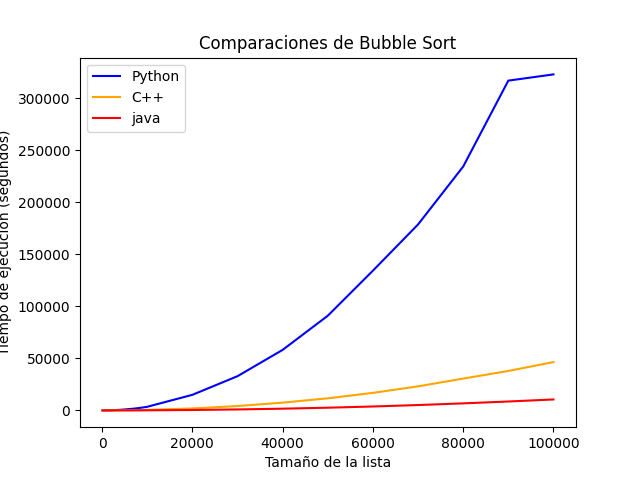
\includegraphics[scale=.60]{img/bubble sort.png}
    \caption{Comparaciones de Bubble Sort en C++,Java y Python}
    \label{fig:primera_figura}
\end{figure}

\subsection{Selection Sort}
Cpp
\lstinputlisting[language=C++]{code/selection.cpp}
Java
\lstinputlisting[language=Java]{code/selection.java}
\vspace{1cm}
Python
\lstinputlisting[language=Java]{code/selection.py}

\begin{figure}[h]
    \centering
    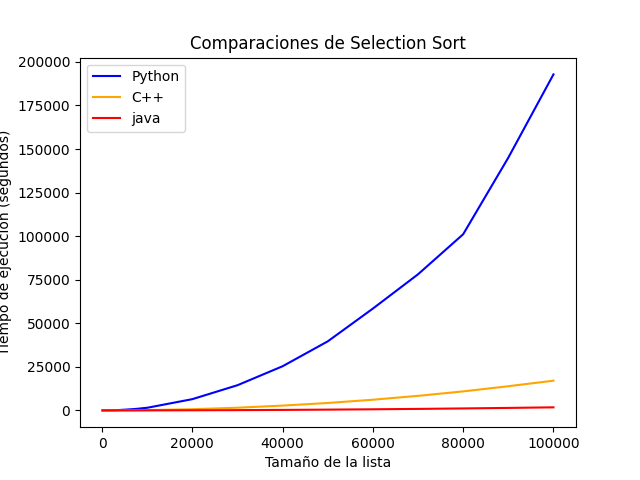
\includegraphics[scale=.60]{img/Selection Sort.png}
    \caption{Comparaciones de Selection Sort en C++,Java y Python}
    \label{fig:primera_figura}
\end{figure}

\subsection{Insertion Sort} 
Cpp
\lstinputlisting[language=C++]{code/insertion.cpp}
Java
\lstinputlisting[language=Java]{code/insertion.java}

\vspace{4cm}
Python
\lstinputlisting[language=Python]{code/insertion.py}

\begin{figure}[h]
    \centering
    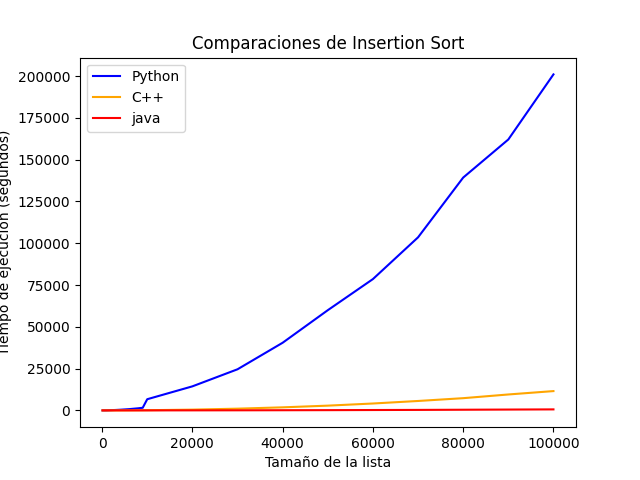
\includegraphics[scale=.60]{img/Insertion sort.png}
    \caption{Comparaciones de Insertion Sort en C++,Java y Python}
    \label{fig:primera_figura}
\end{figure}

\subsection{Counting Sort} 
Cpp
\lstinputlisting[language=C++]{code/counting.cpp}
Java
\lstinputlisting[language=Java]{code/counting.java}
Python
\lstinputlisting[language=Python]{code/counting.py}

\begin{figure}[h]
    \centering
    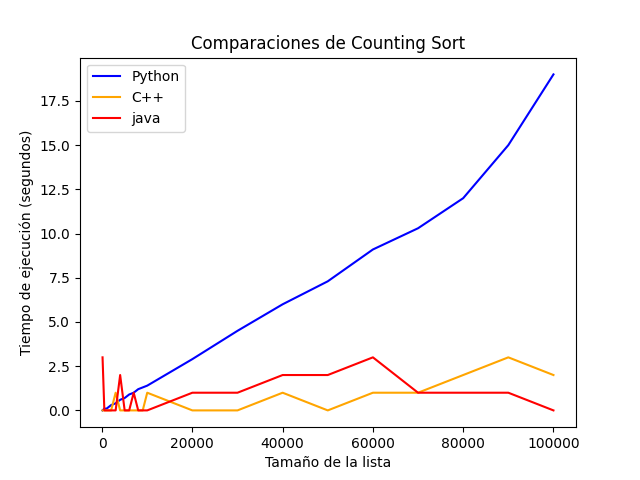
\includegraphics[scale=.60]{img/counting sort.png}
    \caption{Comparaciones de Counting Sort en C++,Java y Python}
    \label{fig:primera_figura}
\end{figure}

\subsection{Heap Sort} 
Cpp
\lstinputlisting[language=C++]{code/heap.cpp}
\vspace{3cm}
Java
\lstinputlisting[language=Java]{code/heap.java}

Python
\lstinputlisting[language=Python]{code/heap.py}

\begin{figure}[h]
    \centering
    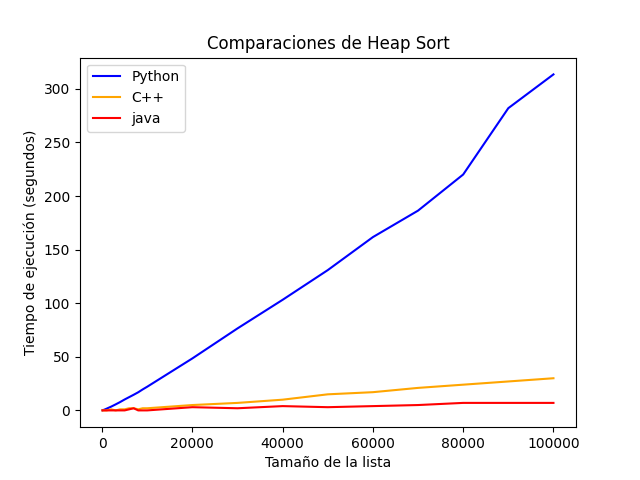
\includegraphics[scale=.60]{img/heap sort.png}
    \caption{Comparaciones de Heap Sort en C++,Java y Python}
    \label{fig:primera_figura}
\end{figure}

\subsection{Merge Sort} 
Cpp
\lstinputlisting[language=C++]{code/merge.cpp}
Java
\lstinputlisting[language=Java]{code/merge.java}
Python
\lstinputlisting[language=Python]{code/merge.py}

\begin{figure}[h]
    \centering
    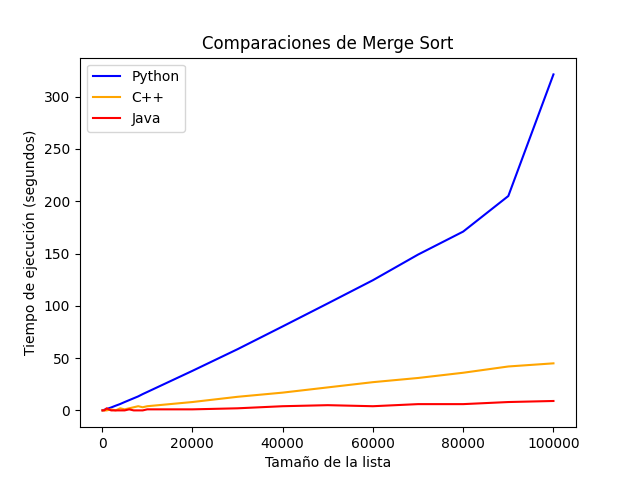
\includegraphics[scale=.60]{img/merge sort.png}
    \caption{Comparaciones de Merge Sort en C++,Java y Python}
    \label{fig:primera_figura}
\end{figure}

\vspace{2cm}
\subsection{Quick Sort} 
Cpp
\lstinputlisting[language=C++]{code/quick.cpp}
Java
\lstinputlisting[language=Java]{code/quick.java}
Python
\lstinputlisting[language=Python]{code/quick.py}

\begin{figure}[h]
    \centering
    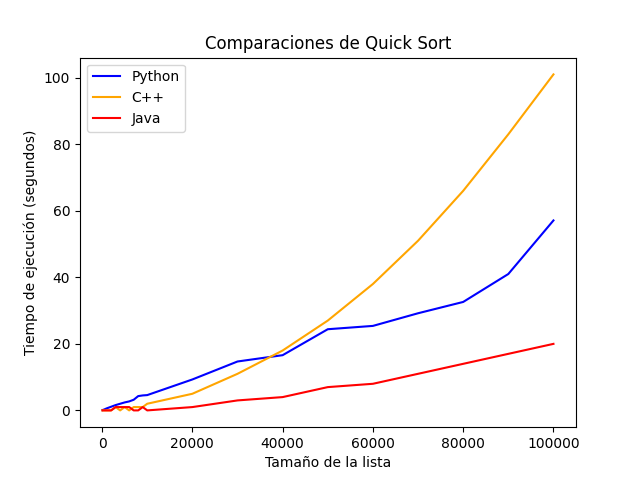
\includegraphics[scale=.60]{img/quick sort.png}
    \caption{Comparaciones de Quick Sort en C++,Java y Python}
    \label{fig:primera_figura}
\end{figure}

Una vez graficados cada algoritmo en cada lenguaje, a continuación se mostrarán los siete algoritmos de ordenación implementados previamente en los tres lenguajes: C++, Java y Python.

\begin{figure}[h]
    \centering
    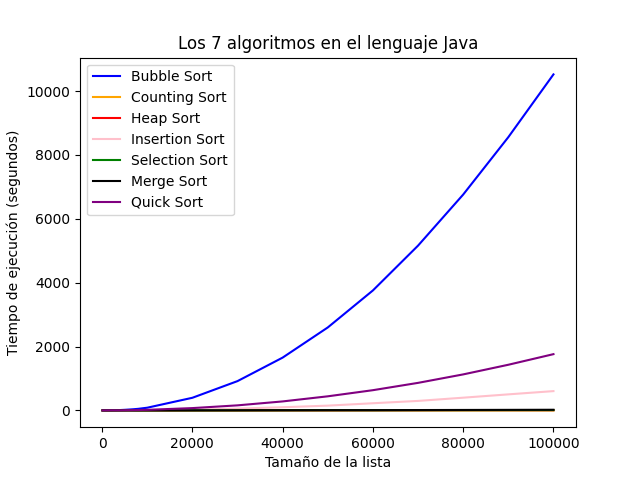
\includegraphics[scale=.60]{img/Java.png}
    \caption{Los 7 algoritmos en Java}
    \label{fig:primera_figura}
\end{figure}

\vspace{2cm}
\begin{figure}[h]
    \centering
    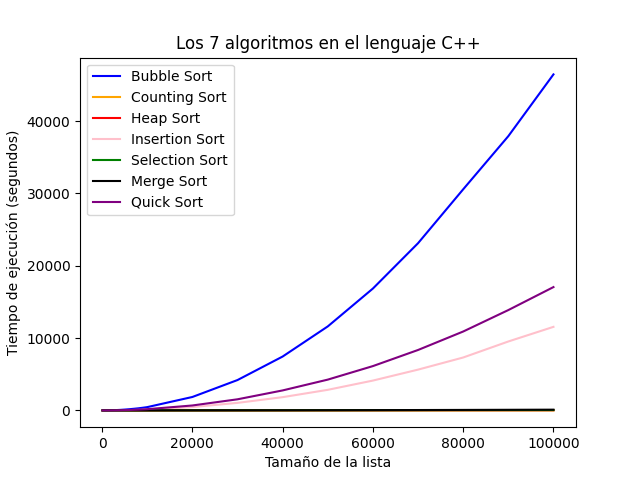
\includegraphics[scale=.60]{img/CPP.png}
    \caption{Los 7 algoritmos en C++}
    \label{fig:primera_figura}
\end{figure}

\begin{figure}[h]
    \centering
    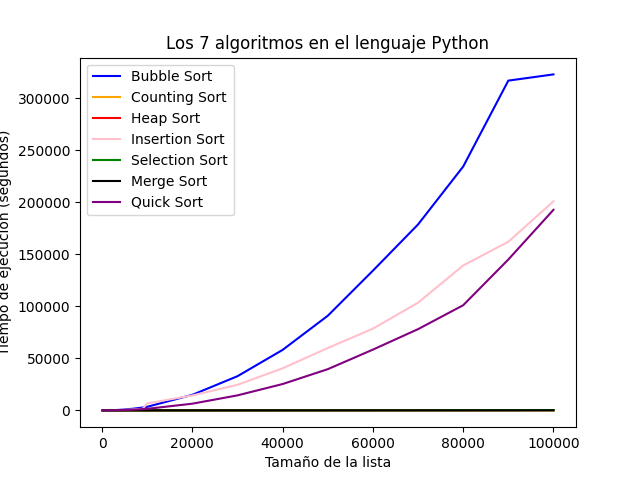
\includegraphics[scale=.60]{img/Python.png}
    \caption{Los 7 algoritmos en Python}
    \label{fig:primera_figura}
\end{figure}

\cleardoublepage
\section{Conclusión}

La presente monografía ha permitido analizar y comparar la implementación de los siete principales algoritmos de ordenamiento, revelando que, aunque cada uno de ellos tiene su propia utilidad, su eficiencia varía significativamente en función del tamaño y la naturaleza de los datos a ordenar. Algoritmos como Quick Sort y Merge Sort se destacan por su capacidad para manejar listas grandes de manera eficiente, mientras que métodos más simples como Bubble Sort, a pesar de su facilidad de implementación, muestran un rendimiento inferior en términos de tiempo de ejecución. 

La elección del algoritmo más adecuado debe considerar el contexto específico de la aplicación; por ejemplo, en situaciones donde se trabaja con conjuntos de datos pequeños o casi ordenados, algoritmos como Insertion Sort pueden resultar más efectivos. Asimismo, es fundamental que los desarrolladores comprendan la teoría subyacente a cada algoritmo, ya que esto les permitirá tomar decisiones informadas que optimicen el rendimiento de sus aplicaciones. 

Este estudio no solo contribuye al entendimiento de los algoritmos de ordenamiento, sino que también actúa como una herramienta educativa valiosa para los estudiantes de ingeniería de sistemas, facilitando una mejor comprensión de la complejidad algorítmica y su impacto en el rendimiento computacional. Finalmente, se sugiere que futuras investigaciones se enfoquen en la implementación de algoritmos híbridos y en la optimización de los algoritmos existentes, así como en su evaluación en diversos entornos de programación y hardware, lo que podría abrir nuevas vías para mejorar la eficiencia en el procesamiento de datos.
\input{content/conclusiones}
\input{content/recomendaciones}


% References
\cleardoublepage
\phantomsection
\addcontentsline{toc}{section}{Referencias}
\nocite{*}  
\bibliographystyle{plain}
\bibliography{ref/ref}



% Appendix
\input{content/Ejemplos.tex}%comentar o quitar este linea de codigo para el trabajo final
\end{document}